\documentclass[pdftex,12pt,a4paper]{report}

\usepackage[pdftex]{graphicx}
\usepackage[ansinew]{inputenc}
\usepackage{geometry}
\usepackage{bbold}
\usepackage{program}
\usepackage[toc,page]{appendix}
\usepackage{subcaption}
\usepackage{url}
\usepackage{textcomp}
\geometry{a4paper,left=2.5cm,right=2.5cm, top=2.5cm, bottom=3cm}
\newcommand{\HRule}{\rule{\linewidth}{0.5mm}}


% definition for ToC

\usepackage{lipsum}% http://ctan.org/pkg/lipsum
\usepackage{titletoc}% http://ctan.org/pkg/titletoc
\titlecontents*{chapter}% <section-type>
  [0pt]% <left>
  {}% <above-code>
  {\bfseries\chaptername\ \thecontentslabel\quad}% <numbered-entry-format>
  {}% <numberless-entry-format>
  {\bfseries\hfill\contentspage}% <filler-page-format>

\begin{document}
\begin{titlepage}

%%LR
\sffamily

\begin{center}


% Oberer Teil der Titelseite:

\includegraphics[width=0.3\textwidth]{logo2.jpg}
\hfill

\includegraphics[width=0.4\textwidth]{logo1.jpg}  
\\[5cm]

{\Large Department of Mathematics}\\[0.5cm]
{\Large Chair of Mathematical Modeling of Biological Systems}\\[0.5cm]
{Technische Universit\"at M\"unchen}\\[2cm]
{\Large Master's Thesis in Bioinformatics}\\[1.5cm]

% Title
\HRule \\[0.4cm]
{ \huge \bfseries Single-cell analysis of cancer drug response using computer vision and learning algorithms on time-lapse microtrench data}\\[0.4cm]

\HRule \\[1.5cm]

{\Large Pandu Raharja}\\[2.5cm]

\vfill
\end{center}
\end{titlepage}
%% THIS REMOVES PAGE NUMBER
%%\pagestyle{empty}

%%LR comprehensive title
\begin{titlepage}
{\sffamily


\begin{center}

\includegraphics[width=0.3\textwidth]{logo2.jpg}
\hfill

\includegraphics[width=0.4\textwidth]{logo1.jpg}  
\\[1.5cm]  

{\Large Department of Mathematics}\\[0.5cm]
{\Large Chair of Mathematical Modeling of Biological Systems}\\[0.5cm]
{Technische Universit\"at M\"unchen}\\[1cm]

{\Large Master's Thesis in Bioinformatics}\\[2cm]
{\textbf{\Large Single-cell analysis of cancer drug response using computer vision and learning algorithms on time-lapse microtrench data}}\\[2cm]
{\textbf{\Large Wirkungsanalyse von Krebsmedikamenten in Einzeller Aufl\"osung durch die Anwendung von Computer-Vision- und Machine-Learning-Algorithmen auf Microtrench- Videoaufnahme}}\\[4cm]

\end{center}
\begin{center}\Large
  \begin{tabular}{ll}
    Author:& Pandu Raharja\\
    Supervisor: &  Prof. Dr. Fabian Theis, Dr. Carsten Marr\\
    Advisor:        &  Prof. Dr. Fabian Theis\\
    & Prof. Dr. Dmitrij Frishman\\
    Submitted:     &  15.12.2017
  \end{tabular}
\end{center}

}% end title page

\end{titlepage}


%%%%%%%%%%%%%%%%%%%%%%%%%%%%%%%%%
% thesis content starts here
%%%%%%%%%%%%%%%%%%%%%%%%%%%%%%%%%

\newpage


\begin{abstract}
Quantitative measurement of cancer drug response is esential to objectively gauge the efficacy of cancer drugs. So far, there has been no method to track and  quantitatively measure single-cell response of of cancer drug treatment. A novel pipeline is presented in this thesis. First, a quasi-high-throughput method to track cells and quantitatively analyze single-cell response to drugs. We investigate the response of model cancer cell lineagues, MOLM and Jurkat, to known anti-cancer drugs Vincristine and Doxorubicine. While the method enabled relatively easy and quasi-high-throughput analysis of cancer treatment \textit{in vitro}, our pipeline could also be adapted in varios contexts involving single-cell analysis with reasonable amount of modifications necessary.
\end{abstract}

\newpage

\tableofcontents

\newpage

\chapter{Introduction}

Cancer is among the deadliest diseases ever known to human being. It is a leading cause of death in 2009, second only to cardiovascular diseases \cite{sudhakar2009history}. The numbers are discontenting, especially in the developed world. In the United States alone, half of men and a third of women are expected to develop some kind of cancer. According to US government, in 2016 alone, an estimated 1,685,210 people will be diagnosed with cancer, while 595,690 more will be die from it \cite{cancergov2017stat}.

Worldwide, the International Agency for Research on Cancer's GLOBOCAN series report that, in 2014, \cite{ferlay2015cancer}.

\begin{verbatim}
I.
- readable to people without background in the fields
- non technical at all
II.
- what have the researches done
-- biologics
-- technicals
III.
thesis overview
4~8 pages
\end{verbatim}

\section{The structure of the thesis}


\chapter{Data and Methods}

As mentioned in previous parts of this thesis: this project consists of three part -- the problem statement regarding the dynamics of cancerous single-cells under pressure of treatment, the microfluidic environment which enables the single-cell protocol and the software implementation used to process and analyze the time-lapse data coming out of the experiment. 

This chapter considers two aspects of the project: the experiment setting and the data analysis pipeline. In the first half of the chapter, we dealt mostly with the experimental background and the underlying questions of single cell dynamics of cancer cell under stress with focus on chemotherapeutic pressure. Henceforth, the cell environment is brought forth. The highlight of this experiment, the microfluidics setup for cell containment, is elucidated in this part. In conjunction with the stup, Some biomedical and biochemistry aspects of the experiment are also mentioned. This includes the drugs and the auxiliary chemicals of interest used in the experiment and the cell lines probed for the experiment. Later on, the hypothesis underlying the experiment is presented.

The second part deals mostly with the quantitative methods and algorithms used to process data into meaningful observations. The part is opened with definitions used in the methods section. Afterwards, each method developed/used in the pipeline is brought forward. For each method, the rationale explaining the reason of using the method is also accompanied in the subsection.

\section{Experimental Setting and Data}

\subsection{Cell Culture}
\label{subsection:cell_culture}

For easier analysis and comparison of experiment resutlts vis-a-vis related experiments, a model cell line is used. In this project, a strain of acute monocytic leukimia (AML) in used: the AML-M5a MOLM-13 cell line. The line used in this experiment derived itself from the cell line initially described by Matsuo \textit{et al} in 1997 \cite{matsuo1997two}. In the paper, the authors developed the line from the peripheral blood of a relapse patient with acute monocytic leukemia (AML) of subtype FAB M5a, which is characterized by predominantly monoblastic leukemia cells in patient sample \cite{arber20162016}. Various studies on the cell lines have made it an ideal candidate for studying \textit{in vitro} study of monocytic differentiation, leukemogenesis and treatment dynamics \cite{matsuo1997two, kelly2002ct53518}.

For the experiment, the acute monocytic leukemia (AML-M5a) MOLM-13 cell line was cultured in Gibco\textsuperscript{\textregistered} RPMI 1640 GlutaMAX medium, produced by Life Technologies \cite{gibcocellculture2017}. The medium is a popular option in human cell biology for experiment and biological synthesis based on human cells and their derivatives \cite{blight2000efficient, shimizu2002fabrication}. It is pre-supplemented with stable form of L-glutamine to prevent ammonia buildup, a common and serious problem in cell culture due to its cell toxicity\cite{satter1974effect}. The medium is further supplemented with Gibco\textsuperscript{\textregistered} Fetal Bovine Serum (FBS), also offered by Life Technologies \cite{gibcofbs2017}, as supplement for the AML-M5a MOLM-13 cell culture.


Some other cell lines were also appraised as potential cell line of interest in this experiment. One of them is Jurkat Cell, a model cell commonly used to study T Cell Leukimia, T cell signalling mechanism and the expression of various HIV-related chemokines \cite{schneider1977characterization}. The cell line was a considered since it is well-studied \cite{johnson2007genome, schena1996parallel}. This is especially true if we consider apoptotic mechanism of the cell line, a problem this project and other related projects by our  and partner labs are trying to investigate. There are several seminal publications about the dynamics of apoptotic mechanism of Jurkat cells we could well compare our results to \cite{gottlieb1996apoptosis}. Samali \textit{et al} \cite{samali1999presence} even studies the dynamics of caspase expression in Jurkat cells, a topic dealt a lot in this project as the chapters progress (see for example Subsection \ref{subsection:treatment}) while Kasai \textit{et al} considers the aspect of spindle checkpoint in the context of apopototic cell death \cite{kasai2002prevalent}. However, we figured out early on that the cell motility of the Jurkat cell line was increased dramatically (a phenomenon observed by others before us \cite{barnhart2004cd95}) upon the introduction of chemotherapeutic treatment -- the increase dramatic enough that the cells managed to escape the microslit it initially landed in.


\subsection{Microfluidics environment}
\label{subsection:microfluid_env}

The general term of microfluidics concerns the wide application of micro-sized devices which hold and control the state of liquid. This includes cell culture medium. There are two categories of microfluidics: active and passive devises. The separation is based on the device's ability to actively manipulate the flow and control of devices. Active devices such as micro-valves can perform sophisticated chemical processes \cite{marsden1993interdisciplinary}. This goes as far as reactions at individual cell level \cite{eyer2012microchamber}. While passive devices, such as micro-arrays, provide a rapid parallel observation platform.

Active microfluidic methods for analysis and manipulation of biological cells have been done in various way and form. In 2003, Wheeler \textit{et al} developed a novel microfluidic device from poly-dimethylsioxane using multilayer soft lithography technology for the analysis of single cells \cite{wheeler2003microfluidic}. The microfluidic setup facilitates the passive and gentle separation of a single cell from the bulk cell suspension. This in turn enables the precise delivery of reagents as little as one nanoliter to the cell. In other use cases, the optical-based microfluidic methods have been used to sort cell with very high accuracy \cite{macdonald2003microfluidic}. This family of method utilizes the fact that different dielectric particles respond differently to an applied light field \cite{tatarkova2003brownian}. Combined with the miniscule spatial setting, the methods are compatible for single-cell resolution analysis. For example, optical-based microfluidic methods have been used to sort cells with very high accuracy \cite{macdonald2003microfluidic, wang2005microfluidic, baret2009fluorescence}.

As a method, passive mocrofluidic methods are mostly used to provide specialized environment in cell-size resoultion. For example, microfluidic settings have been used to keep spatio-temporal identity of single cell for the analysis of the underlying biological dynamics of the isolated cells \cite{mu2013microfluidics, sekhavati2015marker}, which form the methods the design and synthesis of our microtrench environment are based on.

In our cases, the microfluidic settings trace back to the works of our partner lab at Biophysics Department at Ludwig-Maximillians-Universit\"at M\"unchen in 2013 \cite{marel2013arraying} and 2015 \cite{sekhavati2015marker, sekhavati2015dynamic}.

In order to track in a label-free manner non-adherent cells over several generations, we designed and fabricated micro-trenches ($30 \times 120 \, \mu m$) out of PEG-DA (Polyethylene(glycol) Diacrylate), which can accommodate four to six cells. The proposed platform facilitated cell tracking leading to the observation of hundreds of families of cells, derived from one single mother at each case. This enabled us firstly to study the distribution of division times among single cells and also to correlate the division times between sister cells, which are genetically identical. Secondly, the array of micro-trenches enabled the study of the response dynamics of single-cells to doxorubicin, a widely used chemotherapeutic drug, and the comparison of the response to this agent between a chemically synchronized and a non-synchronized population. The detailed methods and protocols for the fabrication of the microfluidics system used in the experiment could be found in Appendix \ref{appendix:microtrench}. The design of the microslit and the schematic representative of cell tracking are seen in Figure \ref{fig:microslit_design}.

The experiment setting looks as follows:

\subsubsection*{The microtrenches:}

The smallest structure of the setting, measuring about 120 microns by 30 microns. The base of the slit is made of Polyethylene (glycol) Diacrylate (PEGDA), an inert substance commonly found as construction material in microfluidics system \cite{sekhavati2015marker}. Each tretment contains about 2400 microtrenches (See \textbf{Results} section) contained in one containment box.

\subsubsection*{The containment system:}

The trench could contain up to 8 cells. The macro-container chosen for containing the wafers holding the microtrenches is ibidi\textsuperscript{\textregistered} sticky-Slide 8 Well (see Figure \ref{fig:ibidi}). In the project, each cell treatment is isolated in one containment box. This ensure the separations of different chemicals used in each treatment. 

\begin{figure}[h]
\centering
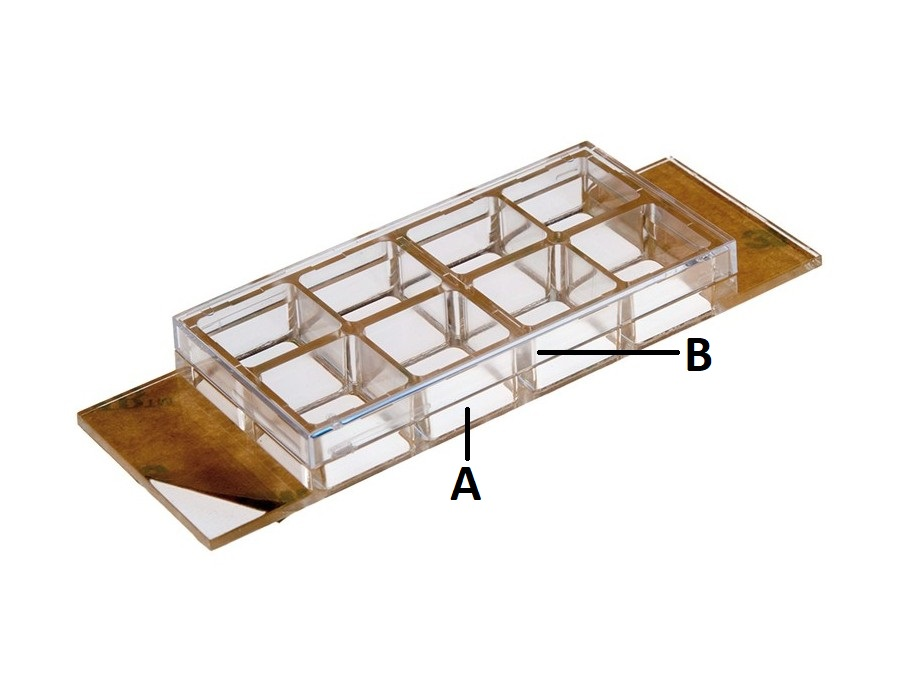
\includegraphics[width=0.6\textwidth]{images/sticky-slide-8-well-marked}
\caption{ibidi\textsuperscript{\textregistered} sticky-Slide 8 Well. The base SU-8 wafer is located in each of the containment box \textbf{(A)}. The SU-8 wafer is then fabricated in the surface of each containment box using nano photolitographic printing. The microfluidics system is then poured and stamped on top the wafer (see Appendix \ref{appendix:microtrench} for detailed manufacturing process). Note that each containment box is upside-open. The cap (\textbf{(B)} is used to prevent the ingress of foreign materials into the medium. \textit{Image taken and modified from ibidi GmbH's website}.}
\label{fig:ibidi}
\end{figure}

\begin{figure}[h]
\centering
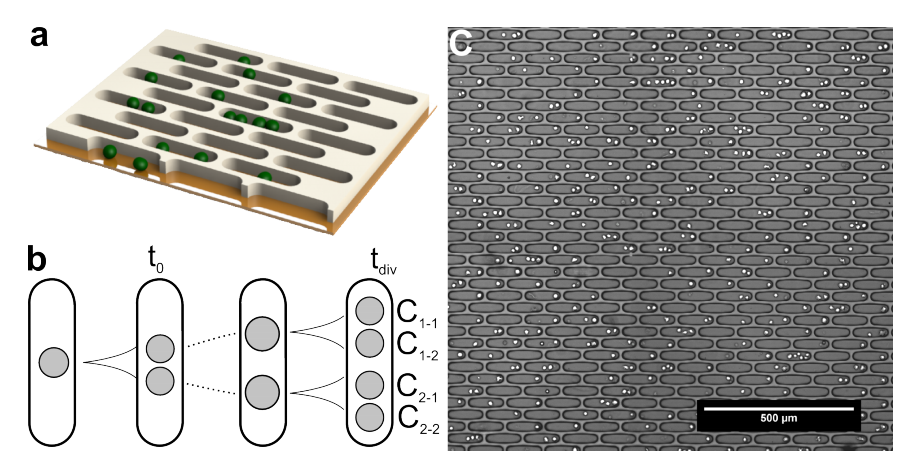
\includegraphics[width=1\textwidth]{images/trenches-sekhavati}
\caption{The structure of microslits: \textbf{(A)} 3D model of microslit on surface with cells inside. \textbf{(B)} The schematic representation of a time-lapse in a trench. First, a singly-placed cell is tracked in a slit. At time $t_0$, the cell divides into two daughter cells. The two cells will be kept tracked until at one point each of the daughter cells will divide at the same time at time $t_{div}$. Note the simplification of the sample. First, not every cell is singly-placed inside a trench. Indeed, not every trench is occupied by cells. Second, not every cell divides. Third, not every cell line observed has three generations in it. And finally, not every children's division times are at the same time. Indeed, this special case almost never happens in real life. \textbf{(C)} The sample view into the environment with cells occupying some slits. Here, the microslits have dimension of 120 $\mu m$ long and 30 $\mu m$ wide. Note also the pointish characteristic of the cells taken in out-of-focus fashion. This improves the performance of the tracking algorithms. \textit{Figure taken from (Sekhavati, 2015) \cite{sekhavati2015dynamic}}.}
\label{fig:microslit_design}
\end{figure}

\begin{figure}[h]
\centering
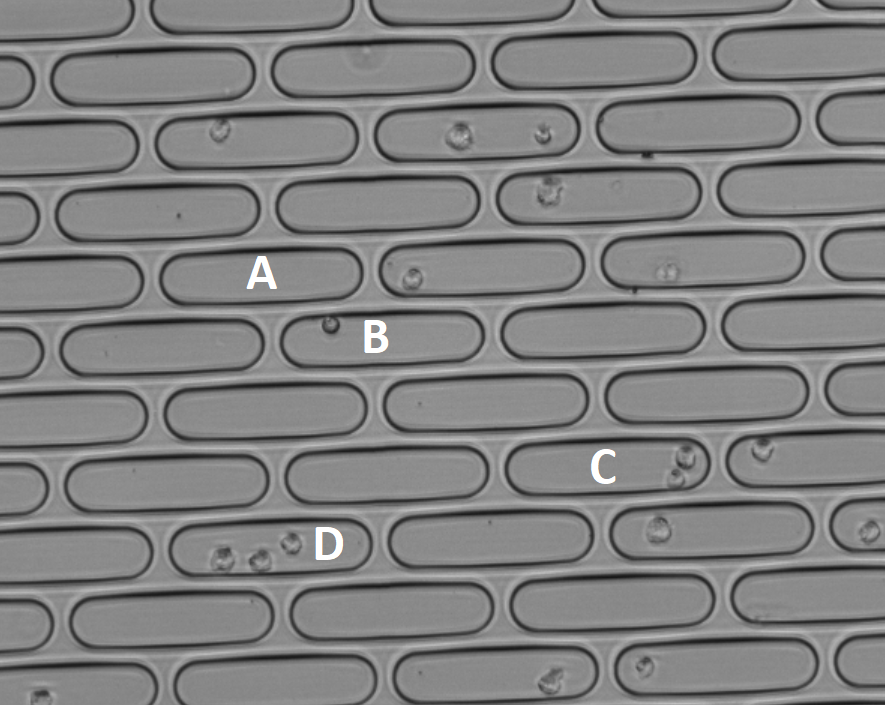
\includegraphics[width=0.8\textwidth]{images/microslit_in}
\caption{The typical view of microslit setting. Some slits contai no cell at all \textbf{(A)}. Several slits contain exactly one cell \textbf{(B)}. A few more slits contain two cells \textbf{(C)} while in rare cases the slit could contain more than two cells \textbf{(D)}.}
\label{fig:microslit_sample}
\end{figure}

\subsection{Cancer Treatment Regimes}
\label{subsection:treatment}

As mentioned in previous chapters, the objective of the project partains mostly the dynamics of single cancer cell under treatment. After mentioning the cell lines of interest (Chapter \ref{subsection:cell_culture}) and the microfluidic setup used to contain cancer cells in single-cell setting (Chapter \ref{subsection:microfluid_env}), we arrived at the last aspect of the experimental seting: the chemical treatment used on the cells.

For cell cultures mentioned in chapter Subsection \ref{subsection:cell_culture}, two treatment regimes are developed : Vincristine and Daunorubicin -- both chemotherapeutic compounds well known for treating various kinds of cancer (TODO cite).

Vincristine is mainly known as Tubulin polymerase inhibitor, a subclass of mitotic inhibitor family of drugs (TODO cite). Mechanistically, it prevent Tubulin polymerization in two ways. First, it binds elongating Tubulin polymer and reduces the affinity of the elongating polymer towards the monomers that are supposed to conjoin the polymer thereby extending it (TOOD cite). Meanwhile, further elongation by the polymers are also prevented via allosteric inhibition -- inhibition caused by spatial occupancy of inhibiting agent -- of polymerating Tubulin via Vincristine (TODO cite). Thus, the effect of Vincristine is most emphasized during the time of high Tubulin synthesis: during the separation of chromosomes in Metaphase by means of tearing them with the simultaneous pulling and pushing mechanism of Tubulin poly- and depolymerization (TODO cite). In the context of chemotherapy, Vincristine is often as combination in CHOP (TODO cite) regime against non-Hodgkin's lymphoma; MOPP, COPP and BEACOPP regimes against Hodgkin's lymphoma; and Stanford V regimes against acute lymphoblastic leukimia (ALL). It is also used to certain degree as immunosuppresant due to its mitotic inhibiting characteristics (TODO cite).

Daunorubicin, like many chemotherapeutic agents including Vincristine, attack cancerous tissues and cells by preventing their division. In comparison to Vincristine however, Daunorubicin prevents the division by disrupting another mechanistic part of cell division: the DNA polymerization. TODO continue 

In normal chemotherapeutic regime, both Vincristine and Daunorubicin are prescribed intravenously to the patients. In our cas, TODO continue.

TODO put pictures on mechanistic action of VCR and Dauno

\section{Definitions}

Mathematical definitions used in the thesis

\subsection{Image Encoding}

Consider the picture of Lenna (Figure \ref{fig:lennasample}).

\begin{figure}[h]
\centering
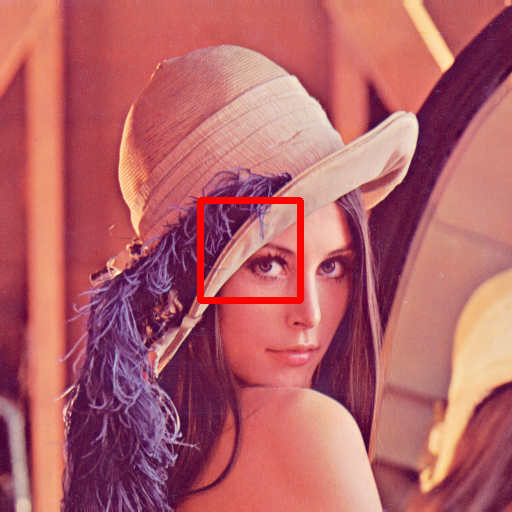
\includegraphics[width=0.5\textwidth]{images/lenna_marked}
\label{fig:lennasample}
\caption{Lenna}
\end{figure}

There are numerous encodings that could be used to internally represent this picture. Many such encodings derived from the so-called Red-Green-Blue (RGB) encodings \cite{sonka2014image}. RGB encoding represents the pixel as a combination of red, green and blue color. This encoding is able to represent various spectra of human visible color and useful enough for most use cases \cite{sonka2014image, jayant1993signal}. To give representation on how the encoding works, the RGB encoding of some part of Figure \ref{fig:lennasample} is shown in Figure \ref{fig:lennas}. For an image of size $m \times n$ pixels, the RGB encoding is thus a 3-dimensional matrix of dimension $m \times n \times 3$. For time-lapsed images accordingly, the RGB encoding of a video of length $T$ is a 5-dimensional matrix of shape $T \times m \times n \times 3$. TODO: put graphical explanation of data here.

%An expansion of such encoding, the RGBH encoding, expands the representation by adding the brightness of the pixel -- known as 'hue'.

\begin{figure}[h]
\begin{subfigure}{.5\textwidth}
  \centering
  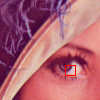
\includegraphics[width=.8\linewidth]{images/lenna_marked_small}
  \caption{1a}
  \label{fig:lennas1}
\end{subfigure}%
\begin{subfigure}{.5\textwidth}
  \centering
  
\includegraphics[width=.8\linewidth]{images/lenna_small}
  \caption{1b}
  \label{fig:lennas2}
\end{subfigure}
\centering
\begin{subfigure}{.5\textwidth}
  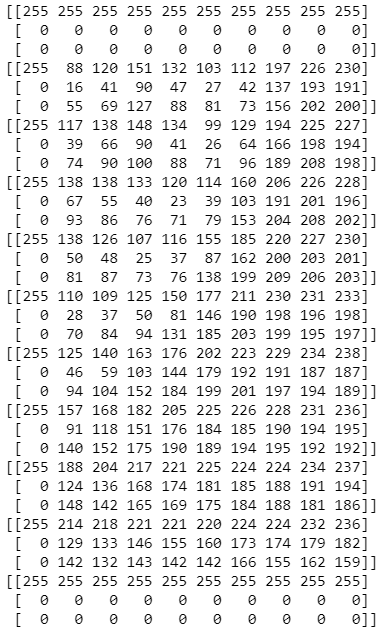
\includegraphics[width=.8\linewidth]{images/lenna_rbg}
  \caption{1b}
  \label{fig:lennas3}
\end{subfigure}
\caption{Figure \ref{fig:lennas1} shows the content of red marked region in Figure \ref{fig:lena}. Figure\ref{fig:lennas2} shows the zoomed part around Lena's right eye and matrix represented in Figure \ref{fig:lennas3} shows the RGB representation of the eye.}
\label{fig:lennas}
\end{figure}

\section{Methods}

\subsection{Laplacian of Gaussian (LoG) Cell Recognition}

\subsection{Shift Correction}

Now, consider a case in which images are shifted in a time-lapsed movie. TODO: explain mechanism. No rotation of camera is assumed, hence there are only two degree of freedoms (vertical and horizontal). Thus, a shift can be defined as a vector movement $\vec{v}$ of all points $x_{i,j} \in M_{t_i}$ in the time-lapse from time $t_i$ to $t_{i+1}$. Given two degrees of freedom and discreteness of the problem due to pixel representation, the task is reduced to finding difference in x- and y-axis ($\delta_x$ and $\delta_y$), so that the difference of transformed pixels at $t_i$ and $t_{i+1}$ are minimized, i.e.:

$$
argmin_{\delta_x, \delta_y} \{d(M_{t_i}, M_{t_{i+1}}^{\delta_x, \delta_y} + (\delta_x, \delta_y)^T)\}
$$

Where $M_{t_{i+1}}^{\delta_x, \delta_y}$ is the entries of matrix $M_{t_{i+1}}$ after applying the shift $\vec{v} := (\delta_x, \delta_y)^T$, i.e.

$$M_{t_{i+1}, \, x, \, y}^{\delta_x, \delta_y} = M_{t_{i+1}, \, x - \delta_x, \, y - \delta_y}$$

For the distance function $d$, the in all channels absolute difference function is used, which is defined as:

$$
d(M_i, M_j) = \sum_{c \, \in \, \{R, B, G\}} \sum_{x} \sum_{y} \vert M_{i, c, x, y} - M_{j, c, x, y} \vert
$$


Since some pixels are lost from the field of view during a shift, only a subset of subsequent pictures is used to determine the shift, preferably those around the center point. This will allow the largest search space possible, since the distance to all four margins of the picture is maximized at the center point. The search for the optimal $(\delta_x, \delta_y)$ pair is implemented as a grid search along the x- and y-axis. An example of the search grid is shown in Figure \ref{fig:searchgrid}.\\

\begin{figure}[h]
\centering
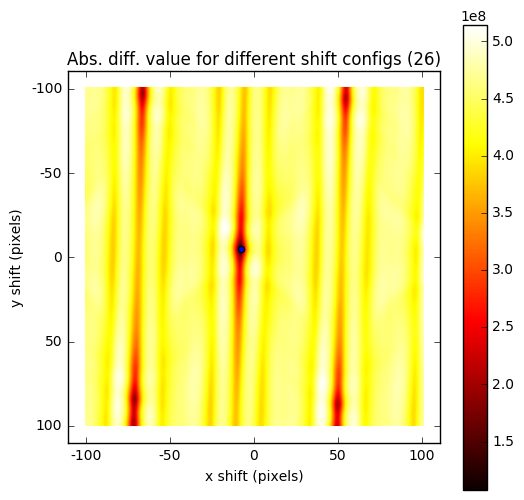
\includegraphics[width=0.5\textwidth]{images/search_grid}
\caption{Search grid shift for Position 26. The search was conducted for shift between the last time point before and the first time point after the drugs treatment. The minimum is marked with thick black dot, which is returned after every grid-search call as inferred shift. In the position, the shift was inferred to be 8 pixels upwards and 5 pixels leftwards. Notice the repeating pattern of relatively favorable configurations after approximately 50 horizontal and 100 vertical pixels caused by lattice nature of the slits.}
\label{fig:searchgrid}
\end{figure}

%% TODO: RESTRUCTURE THE CHAPTER

Since the time-lapsed data consists mainly of grayscale image, the RGB encoding could be the directly transformed to grayscale encoding. Using the transformed method also speeds up the calculation process since the distance function only computes the difference of grayscale channel's values:

$$
d(M, N) =  \sum_{x} \sum_{y} \vert M_{c, x, y}^{gray} - N_{x, y}^{gray}\vert
$$

Due to lost pixels around the margin of before and after pictures, only the overlapping part of both slides are included after the correction. Thus, for an inferred shift of $(\delta_x, \delta_y)$, the new dimension of the pictures is then $(m - \delta_x) \times (n - \delta_y)$. This change would then propagation to the other time-lapse images to maintain consistency of the images.\\

Ideally, the shift correction should be done for each position to reduce the track dropout rate caused by image shifts. This is however computationally very expensive and, as seen in Figure \ref{fig:pixdiff}, not really necessary since the biggest shift indeed only happens right before and after the treatment, as it was expected during the experiment setting. As seen in Chapter XX (TODO: quote), the tracking allows certain amount of tolerance. In this regard, the other frame shifts are way within the tolerance of our tracking algorithm. As shown in Figure YY (TODO: add droput rate), the dropouts caused by frame shifts in the other time points are basically noisy dropout caused by random noise in time-lapse movie being tracked as cells \cite{jaqaman2008robust}.

The algorithm for shift inference is available in Appendix \ref{appendix:algo}.

\begin{figure}[h]
\centering
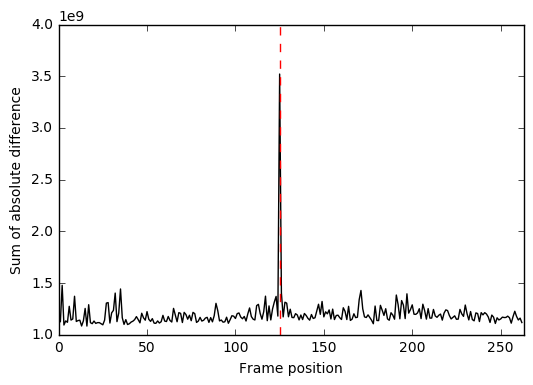
\includegraphics[width=0.8\textwidth]{images/pixdiff}
\caption{Pixel difference between consecutive frames at Position 26. In most cases, the pixel difference between the frames is mainly caused by moving cells. The diference during the treatment, on the other hand, is caused by physical shift of the frame. While moving cells mostly caused minimum noise-like pixel difference, the physical shift of field of view distorts the physical alignment and evokes immense pixel difference.}
\label{fig:pixdiff}
\end{figure}

\subsection{Cell death signals}

Measuring cell death is a crucial part of the experiment, as the reliable determination of it is the basis of most analysis in this thesis. There are several way to measure cell deaths with varying complexity and accuracy. Each method contains certain assumptions of cell death.\\

For example, determining cell death by cell movement assumes death of a cell if no movement beyond random flux is observed in certain amount of time. This obviously has certain drawbacks, such as when the observation is done in non-static environment. Moreover, defining the limit of the random flux, above which a given cell is assumed to actively move, is not a trivial task. Some kind of gold standard for a given cell line and environment has to be established manualy, which is very time consuming. This fact is again made even more complicated by the fact that many cells show different movement pattern upon introduction of treatment. It is well known that some cells tend to move faster or slower under stress, the situation many cancerous cells in our experiment will experience upon addition of cancer drugs treatment \cite{pienta1991effects, fenteany2003small, ruocco2012suppressing}.\\

The second method is using cell size. During apopotosis, the cells would shrink. Given It is known that cell size TODO continue.

In this experiment, two cell signals are used as indicator of cell death. TODO continue

\chapter{Analysis Pipeline}

\chapter{Results}

\begin{verbatim}
I. Pipeline

II. Quantitative Analysis
\end{verbatim}

\chapter{Summary and Outlook}

\begin{verbatim}
I. Summary (and discussion?)
Connect Results with Background

II. Outlook
Improvemnt capability
\end{verbatim}

%% BIBLIOGRAPHY %%

\bibliographystyle{unsrt}
\bibliography{mabib}

%% APPENDICES %%

\begin{appendices}

\chapter{Annex: Methods}

\section*{Micro-trenches array fabrication} \label{appendix:microtrench}

\subsection*{Photolithography of the SU-8 wafer}

The fabrication of the SU-8 (MicroChem Corp, USA) wafer was executed in a in-house cleanroom facility using a ProtoLaser LDI system (LPKF Laser \& Electronika, Naklo, Slovenia), with a 375 nm wavelength laser and 1 μm spot diameter.

\subsection*{Softlithography and Micromolding}

Polydimethylsiloxane (PDMS) prepolymer solution is mixed with the crosslinker in a 10:1 ratio (w/w) (Sylgard 184, Dow Corning, USA) and then degassed under vacuum. PDMS is then purred on the SU-8 wafer, degassed and cured in 50 oC. The resulting PDMS stamp is peeled off the wafer and cut into appropriate shapes. The PDMS pieces, with 25 1/4 pillars in height, are activated with argon plasma and then immediately placed upside down on a silanized with TMSPMA (3-(Trimethoxysilyl)propyl methacrylate, Sigma-Aldrich) glass coverslip. A solution of PEG-DA (Mn=258) containing 2\% v/v of the 2-hydroxy-2methylpropiophenone (both from Sigma-Aldrich, Germany) is freshly prepared and then a drop is deposited at the edge of the PDMS stamp. The PDMS stamp is filled by capillary force induced flow. PEG-DA is then polymerized in an UV-ozone cleaning system (UVOH 150 LAB, FHR, Ottendorf, Germany). Next, the PDMS stamps are peeled off and the resulting micro-trenches of cross-linked PEG-DA are dried in an oven (Binder GmbH, Tuttlingen, Germany) overnight at 50oC. Finally, the slides are sonicated with 70\% ethanol and distilled water before a sticky slide is attached on top (8-well sticky slide, ibidi GmbH, Munich, Germany).

\chapter{Algorithms}\label{appendix:algo}

\section*{Shift Inference} 

\begin{verbatim}
def infer_shift(last_slide, first_slide, search_space=(200, 200)):
    
  if (search_space[0] % 2 != 0) or (search_space[1] % 2 != 0):
    print("Search spaces have to be even!")
    return None
  else:
    
    ## calculate absolute difference for various shifts
    x1 = search_space[0]
    x2 = search_space[0]
    y1 = search_space[1]
    y2 = search_space[1]
    mid = f1.shape[0] // 2, f1.shape[1] // 2
        
    ## results storage        
    absdiffs = np.zeros((search_space[0] + 1, search_space[1] + 1))

    ## last slide before treatment
    f1sub = f1[(mid[0] - x1):(mid[0] + x2), (mid[1] - y1):(mid[1] + y2)]
    
    ## search space 
    xdiff1 = -int(search_space[0] / 2)
    xdiff2 = int(search_space[0] / 2) + 1
    ydiff1 = -int(search_space[1] / 2)
    ydiff2 = int(search_space[1] / 2) + 1
    
    for xdiff in range(xdiff1, xdiff2):
      for ydiff in range(ydiff1, ydiff2):
      
        ## calculate absolute difference for shift
        f2sub = f2[(mid[0] - x1 + xdiff):(mid[0] + x2 + xdiff), 
                   (mid[1] - y1 + ydiff):(mid[1] + y2 + ydiff)]
        x = xdiff + int(search_space[0] / 2)
        y = ydiff + int(search_space[1] / 2)
        absdiff_xy = np.sum(cv2.absdiff(f1sub, f2sub).ravel())
        absdiffs[x][y] = absdiff_xy
        
        
    ## calculate shift based on calibration data
    x = np.argmin(absdiffs) // absdiffs.shape[0]
    y = np.argmin(absdiffs) % absdiffs.shape[0]
    
    """
    True shift is the opposite of coordinate encoded
    in absdiff
    
    Let X2 the second picture and X1 the first picture.
    If the sub-picture of first slide of X2 centered
    at (c1 + s1, c2 + s2) fits the most with the sub-picture
    of the last slide of X1 centered at (c1, c2)
    then the pictures shift by (-s1, -s2) upon treatment
    """
    diff = -(x - search_space[0] / 2), -(y - search_space[1] / 2)

    return diff
\end{verbatim}

\end{appendices}

\end{document}